\label{Implementierung_Ablauf}
\subsection{Umsetzung Graph}
\begin{frame}
\begin{center}
\begin{footnotesize}
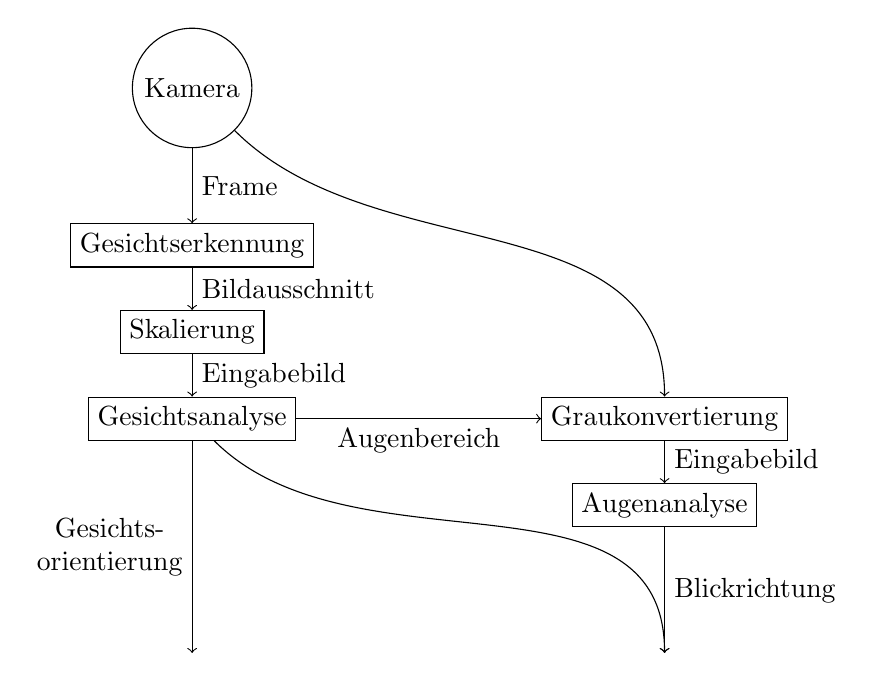
\begin{tikzpicture}
	\node[circle,draw,align=center] (C) at(0,0) {Kamera};
	\node[draw,align=center] (F) at(0,-2)  {Gesichtserkennung};
	\node[draw,align=center] (S) at(0,-3.1)  {Skalierung};
	\node[draw,align=center] (G) at(6,-4.2)  {Graukonvertierung};
	\node[draw,align=center] (A) at(0,-4.2)  {Gesichtsanalyse};
	\node[draw,align=center] (E) at(6,-5.3)  {Augenanalyse};
	
	\node (outA) at(0,-7.3)  {};
	\node (outB) at(6,-7.3)  {};
	
	\draw[->] (E)to node[right,align=center]{Blickrichtung}(outB);
	\draw[->] (A)to[out=-45,in=90] node[right]{}(outB);
	
	\draw[->] (C)to node[right]{Frame}(F);
	\draw[->] (F)to node[right]{Bildausschnitt}(S);
	\draw[->] (S)to node[right]{Eingabebild}(A);
	\draw[->] (A)to node[left,align=center]{Gesichts-\\orientierung}(outA);
	
	\draw[->] (A)to node[below]{Augenbereich}(G);
	\draw[->] (C)to[out=-45,in=90] node[left]{}(G);
	\draw[->] (G)to node[right]{Eingabebild}(E);
\end{tikzpicture}
\end{footnotesize}
\end{center}
\end{frame}
Zur Bestimmung der Blickrichtung sowie Kopfposition und Orientierung wird ein mehrstufiges Verfahren eingesetzt:\\
Zuerst müssen alle Gesichter, die im aktuellen Videobild (Frame) vorhanden sind, detektiert werden mit MTCNN-Face, siehe \autoref{MTCNN}. Dabei machen die relevanten Bereiche nur einen sehr geringen Anteil des gesamten Bildes aus.\\
Ist ein Gesicht in mehreren Einzelbildern des Videos abgebildet, so muss auch eine Identitätszuordnung vorgenommen werden, damit dem Computerprogramm bekannt ist, welches Gesicht in Bild 1 welchem in Bild 2 entspricht. Für die Zuordnung reicht es meist aus, jene Box zu wählen, die am ehesten den selben Bildausschnitt repräsentiert. Entweder über ähnliche Positionierung im Videobild oder über die Bildähnlichkeit, da ein Kopf sich zwischen zwei schnell aufeinanderfolgenden Einzelbildern nur limitiert bewegen kann.\\
Damit sicher auf allen Gesichtern gerechnet werden kann, ist eine semiautomatische Korrektur erforderlich um Falsch-Detektionen zu entfernen und fehlende Boxen der Gesichter ergänzen zu können. Daher können alle bisher unternommenen Schritte auch von anderen Verfahren übernommen werden, da es sich hierbei nur um einen Vorverarbeitungsschritt handelt und zur Beschleunigung sowie Stabilität der späterer Berechnung beitragen soll.\\
Die Bereiche müssen nicht exakt sein, da OpenFace einen eigenen Facedetector besitzt.\\
Je nach verwendetem Trainingsdatensatz und darin enthaltener Annotation werden z.B. Kinn und Haaransatz noch als Gesichtsbereich oder schon als außerhalb des Gesichtes betrachtet wodurch  Gesichtserkennung und Landmark Erkennung auf unterschiedlichen großen Gesichtsbereichen arbeitet. So geben beiden Methoden (OpenFace und MTCNN-Face) Boxen aus, diese sind in ihren Ausmaßen allerdings nicht identisch. Da die folgende Verarbeitung eine OpenFace-skalierte Box erwartet, ist ein Zwischenschritt zur Vergrößerung der erkannten Bereiche notwendig, damit das gesamte Gesicht abgebildet ist. Für die MTCNN-Face Box hat sich eine Vergrößerung um $30\%$ als sinnvoll erwiesen, um Ungenauigkeiten bezüglich der Position und Dimension des Kopfes im Bild entgegen zu wirken.\\
Damit das Verfahren im nächsten Schritt zuverlässig arbeiten kann, werden alle zu kleinen Bildbereiche hochskaliert, um die Gesichter auf eine Mindestgröße zu bringen, siehe \autoref{scale_Algos}\\ Die von MTCNN gelieferten und vergrößerten Boxen werden auf eine Breite von 130 Pixel gebracht (100 Pixel für den Kopf mit $30\%$ Rand durch Vergrößerung), damit das beinhaltete Gesicht auf der gewünschten Größe dargestellt wird. Der Skalierungsfaktor ist für jeden Bildausschnitt individuell und kann sich über die Zeit ändern, wenn sich z.B. die Distanz zwischen Person und Kamera ändert.\\
Von einer zu starken Vergrößerung ist abzuraten, da sich der Rechenaufwand pro Gesicht erhöht und die Zuverlässigkeit der Berechnungen von OpenFace sinkt, z.B. durch Falschdetektion. Neben der Skalierung des Bildausschnittes muss bekannt sein, wie Punkte im skalierten Bildausschnitt in das Frame überführt werden können, damit dies bei späteren Berechnungen berücksichtigt wird.\\
Auf diese zuvor bestimmten und vergrößerten Bildausschnitten werden nun von OpenFace weiterverarbeitet um die Landmarks, die signifikanten Punkte eines Gesichtes zu bestimmen, siehe \autoref{OpenFace}.\\
Durch die vorherige Identitätszuordnung der Gesichter kann das Verfahren gezielt auf einzelnen Personen arbeiten und ein entsprechend auf die Person eingestelltes CLNF verwenden, um bessere Ergebnisse zu erzielen, auch für jene Personen die nur selten dargestellt sind. Außerdem können alle gefundenen Personen gleichzeitig (parallel) ausgewertet werden und durch die zuvor bestimmten Bildbereichen in denen ein Gesicht zu sehen ist, kann unnötige Suche vermieden werden.\\
Für die eigentliche Bestimmung der Landmarks bietet OpenFace zwei verschiedene Methoden, die Berechnung auf Bildern und Videos. Dies ist interessant für die spätere Anwendung, da somit auch Einzelbilder verwendet werden können, die eine deutlich höhere Auflösung besitzen als ein Video.\\
Der Hauptunterschied zwischen den beiden Verfahren ist das Lernen, dass bei der Videoauswertung verwendet wird, wodurch sich der Toleranzbereich deutlich erhöht und bessere Ergebnisse geliefert werden und, sollte ein Gesicht im aktuellen Frame erfolgreichen detektiert werden, können auch die nachfolgenden Frames durch das Lernen ausgewertet werden. Dies liegt an der Anpassung des Modells und dem möglichen Tracking der Landmarks.\\
Dennoch kann es passieren, dass trotz allem ein Gesicht falsch detektiert wird, wie z.B. das Erkennen eines sehr kleinen Gesichtes innerhalb einer Ohrmuschel. In solch einem Fall muss das CLNF zurückgesetzt werden, damit sich der Fehler nicht fortpflanzt.\\
Für den im nächsten Schritt verwendeten ElSe Algorithmus muss der Bildausschnitt des Auges in ein Graubild umgewandelt werden, siehe \autoref{Graubild}.\\
Für die Bestimmung der Blickrichtung ist vor allem das Zentrum der Pupille bzw. Iris ausschlaggebend. Das Zentrum ergibt sich aus dem Umrissen (Landmarks) der Pupille bzw. Iris und muss möglichst exakt bestimmt sein, daher müssen diese aus dem Ergebnis von ElSe abgeleitet werden, siehe \autoref{ElSe}.\\
Da die Berechnung unabhängig der Landmarks ausgeführt wird, empfiehlt sich das Ergebnis zu überprüfen, damit die bestimmten Landmarks auch innerhalb der Augenhöhle liegen und grobe Fehler vermieden werden.\\
Nun wird auf Basis der Landmarks und Kameraparameter die Position und Orientierung der Gesichter sowie die Blickrichtung bestimmt, siehe \autoref{calc_Position}.